\chapter{Requirements Analysis}
\label{chapter:requirements-analysis}
\minitoc\vspace{.5cm}
Based on the fundamentals, the requirements for the prototype to be developed will be formulated in this chapter.
Thereby, relevant aspects for the specific implementation will be considered.
The analysis, the creation of requirements and the commitment from all sides to these requirements are important steps to successfully realize a project, not only in the software development area.
Each step has to be discussed and approved by a representative of the \ac{FOKUS}.
Due to the fact that the prototype will be created from scratch, most of the concepts have to be created in brainstorming meetings.
An agile development process will be used to react to rapidly changing requirements.
As mentioned before a Kanban like method will be used in this project.


\section{Functional requirements}
\label{section:functional-requirements}
% virtualization
As the fundamental requirement, the prototype to be developed has to create, manage and maintain virtualized containers on a fog node.
Tools like Open Baton inherently support OpenStack as the \ac{ETSI} \ac{MANO} \ac{VIM} layer.
Most \ac{MANO} tools like Open Baton use OpenStack, which deploys virtual machines to virtualize the \acp{NF}.
This is a rock solid solution for a cloud environment.
Unfortunately, a bare-metal virtualization is most of the time not feasible on small power devices like they are used in the \ac{IoT} area.
Therefore, a much more efficient and lightweight solution, like container virtualization, should be used and handled by an orchestration engine.
The desired service, like a \ac{NF}, can be bundled in one or multiple containers and executed afterwards on the expected \ac{IoT} nodes.
Such a bundle of containers should be passed to the node as a build plan or a blueprint of the service.
The fog node engine should accept the blueprint and deploy the containers to the desired virtualization layer.
Afterwards, the lifecycle of the services should be monitored.

% constraints
The second functional requirement is the implementation of a constraint logic, which will be used to filter relevant nodes during the orchestration.
A constraint can be a functional and non-functional capability.
For example, this could be a specific hardware component, like a sensor or a ZigBee dongle, which is necessary to execute the \ac{NF} or a hardware requirement, like \ac{CPU} power, \ac{RAM} or disk space.
It could also be a non-functional constraint, for example a specific software, which has to be installed or a protocol, that can be used.
The engine should be able to manage these constraints by itself and if necessary for all adjacent nodes and should consider them while choosing a suitable node for the desired \ac{NF}.
The whole functionality should work similar to the labels in Docker Swarm.
Therefore, a Docker Swarm node can have multiple labels, which can be considered when deploying an image.
This behavior should be achieved by the fog node engine.

% lifecycle
Another important aspect is the lifecycle management of the node, the deployed services and images.
In the prototype it has to be elaborated how the lifecycle of the several components can be implemented.
An sample implementation of a node management lifecycle is shown in the OpenFog Reference Architecture for Fog Computing\autocite[cf.][p. 52 f.]{OpenFog:2017}.
Figure \ref{fig:open_fog_node_mgm_lifecycle} describes the five steps of a typical lifecycle based on these architecture.
\begin{figure}[H]
    \centering
    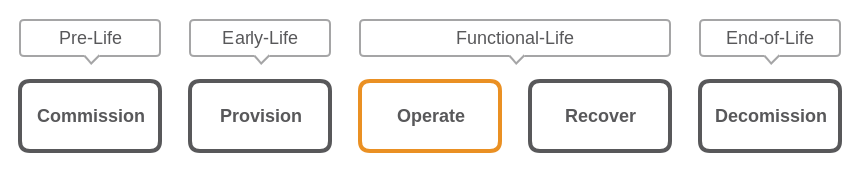
\includegraphics[width=\textwidth]{resources/images/node_management_lifecycle.png}
    \caption[Node management lifecycle]{Node management lifecycle. Adapted from: \autocite[p. 52]{OpenFog:2017}}
    \label{fig:open_fog_node_mgm_lifecycle}
\end{figure}

\begin{itemize}
  \item The \textbf{Commission} is the earliest phase in a lifecycle mostly used to perform action like identification, certificates or calibration of time.\autocite[cf.][p. 52 f.]{OpenFog:2017}
  \item In the \textbf{Provision} phase the node will be enrolled to the system so that the node can be discovered and identified and also advertises features and capabilities.\autocite[cf.][p. 52 f.]{OpenFog:2017}
  \item The \textbf{Operate} phase is the state of the node when everything operates normal.
  This includes the reliability, availability and serviceability of the node.\autocite[cf.][p. 53]{OpenFog:2017}
  \item In contrast to that the \textbf{Recover} phase performs action if something operates out of norm.\autocite[cf.][p. 53]{OpenFog:2017}
  The node should be able to recover to the normal state.\autocite[cf.][p. 53]{OpenFog:2017}
  \item Finally the \textbf{Decomission} phase is used for cleaning up sensitive data on the node and to unregister from other components.\autocite[cf.][p. 53]{OpenFog:2017}
\end{itemize}

In addition to the node lifecycle, an exemplary lifecycle for services and images is shown in the \ac{ETSI} \ac{MANO} specification\autocite[cf.][p. 67 ff.]{ETSI:MANO:2014}
This lifecycle handles several state from the instantiation of a service, further querying some data, up to the termination of service.
Some of the specifications are tightly coupled to \acp{NFV}.
However, this lifecycle specification is a good starting point to elaborate a custom solution.

% GUI
The last functional component to be developed will be the \ac{GUI}.
This should only be used to demonstrate the basic functionalities of the prototype.
It is not designed to use it in production.
Therefore, the \ac{GUI} will not have any security mechanisms like authorization, authentication or user management.
This includes that existing nodes will be displayed with all the related services.
Additionally, it can be used to deploy new services while using the existing endpoints.

% secondary conditions
Some secondary conditions should also be fulfilled.
The whole system should be modular and easy to extend.
Modules should be as decoupled as possible and the whole system should be controlled via an \ac{API}.
The centralized cloud environment should be easily replaceable and should not be exclusively bound to Open Baton or any other tool.
It also applies to the prototype, it should not be bound to Docker only and should be able to use other virtualization tools.
Finally, the whole system should be well tested and documented.


\section{Non-Functional requirements}
\label{section:non-functional-requirements}
The non-functional requirements are also addressed and they are classified into the following categories:

\paragraph{Reliability:} Due to the fact that the final product will only be a prototype and has only a few development iterations, it will not be production ready. Nevertheless the prototype will be developed with stability and robustness in mind and the code will be well tested and documented.
\paragraph{Performance:} As a crucial requirement, extra attention will be payed for making the application as lightweight as possible and reduce the dependencies and tool chain.
The use of powerful but resource consuming tools and libraries, like huge databases or message queues, will be renounced.
Necessary libraries will be used if they are essential, but in general they will be selected with the requirement of being executed on low power devices.
\paragraph{Usability:} The prototype should be easy to use, to install and to maintain.
An easy to use installation script will be developed.
The source code will be well documented and an user guide will be created.
\paragraph{Maintainability:} Due to the fact that the prototype will be a solid base for further development, it will be created as modular as possible.
It should also be well structured by using well known design patterns.
Each component should be easy to replace and also easy to maintain.
The project should be open source and extensible by everyone.
Code tests and code style checks will help to ensure the functionality and extensibility of the application.
\paragraph{Security:} Also an important part as in nearly every project, security will be considered.
Especially in the \ac{IoT} security becomes important due to several bad examples in the last years\footnote{\url{https://www.corero.com/resources/ddos-attack-types/mirai-botnet-ddos-attack.html}}\footnote{\url{https://security.radware.com/ddos-threats-attacks/brickerbot-pdos-back-with-vengeance}}.
Therefore, particular scenarios will be considered and recommendations will be addressed.
The focus of the prototype will be on showing up the functionality of the application, without implementing security related mechanisms right down to the latest detail.
\paragraph{Correctness:} As mentioned before the code will be tested and code style checks will help to have a standardized code base.
\paragraph{Flexibility:} The software will be developed with some well known standards in mind, like the \ac{MANO} specification, standard protocols and also design patterns, to make the source code more readable and understandable.
This makes it easier to add new or replace existing components.
\paragraph{Scalability:} The prototype will also be developed to be executed on several nodes at the same time.
Primary usage will be in a cluster with several other nodes.
This need will be considered during the whole development phase.


\section{Use-Case-Analysis}
\label{section:use-case-analysis}
This analysis will show up four exemplary use cases of the prototype to be developed.
These use cases describe the system in a simplified and abstract manner.
They will not refer to any technology, but will show up the usage of the prototype from a user perspective.

\paragraph{Service deployment from a cloud orchestrator:}
It will be the most common use case in this consideration.
A service, for example a \ac{NF}, should be deployed to a single node.
Figure \ref{fig:use_case_deploy_service} illustrates this use case.
Therefore, the prototype will be installed on the node itself.
A cloud service, such as Open Baton, will orchestrate the deployment.
In doing so, a so called blueprint, which is basically a description of the service, the images and the capabilities that are necessary to execute the image, will be passed over to the prototype via an \ac{API}.
The prototype will receive and parse them afterwards.
All the provided images will be executed on the same node and at the end the service is up and running.
The state of the services can be observed at any step of the process.

\begin{figure}[H]
    \centering
    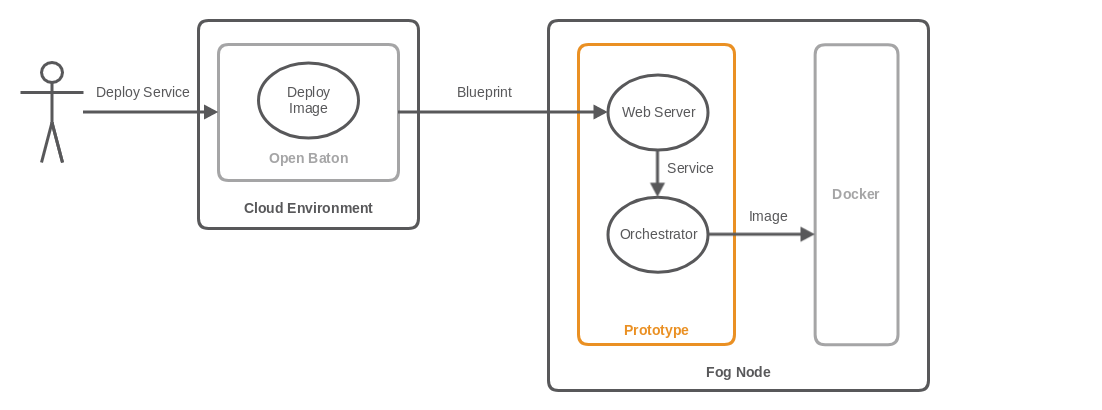
\includegraphics[width=\textwidth]{resources/images/use_case_deploy_service.png}
    \caption[Use case: Service deployment from a cloud orchestrator]{Use case: Service deployment from a cloud orchestrator}
    \label{fig:use_case_deploy_service}
\end{figure}

\paragraph{Service deployment based on capabilities:}
Also in this case a cloud service like Open Baton will deploy a service to a node cluster.
Figure \ref{fig:use_case_deploy_service_multiple_nodes} illustrates this use case.
Again, one node will get the blueprint and parse it.
Each image has labels, hereinafter called \textit{capabilities}, attached to it.
During the parsing of the blueprint, the application is checking, if the node can fulfill all of these \textit{capabilities}.
If an image can not used by this node, the application will search for a node, that is able to deploy the image.
For example, if one image needs a ZigBee dongle to measure data, than the capability \textit{ZigBee} is added to the image in the blueprint.
The first node, Node A, has no ZigBee dongle connected and therefore, it is not able to fulfill that requirement.
Node A will then ask all the other nodes in the cluster, if they can satisfy the need.
Node B will respond that it is also not able to do so.
Node C is able and will respond with a related message.
Node A sends over the image to be deployed and Node C will execute it.
From that point on, Node A is still responsible for the whole service, but Node C is executing the container that was started from the image and will frequently be asked for the state of the container.
This process can be repeated for one or multiple images.
If each image was deployed, the service is up and running and can be observed again by the user.

\begin{figure}[H]
    \centering
    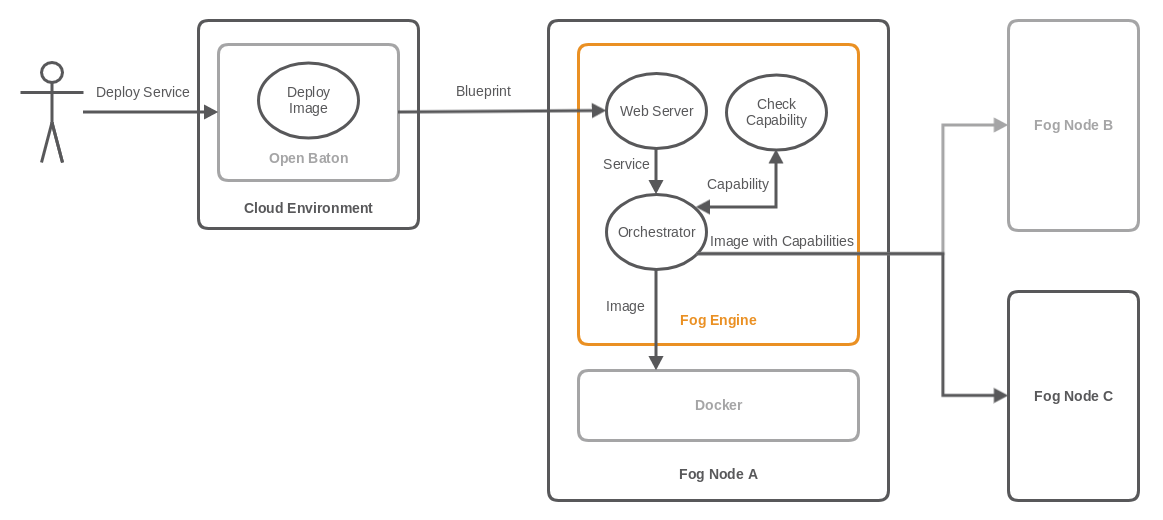
\includegraphics[width=\textwidth]{resources/images/use_case_deploy_service_multiple_nodes.png}
    \caption[Use case: Service deployment based on capabilities]{Use case: Service deployment based on capabilities}
    \label{fig:use_case_deploy_service_multiple_nodes}
\end{figure}

\paragraph{A new node will appear:}
If a new node will be added to the cluster, all the other nodes should be informed about this circumstance.
Therefore, the appearing node will send out a message with some meta information to the broker, with for example the \ac{IP} address of the node, that send it to all the other nodes.
Each node in the cluster will get the message and can store the information.
Additionally, the nodes will also send back a message with their meta information.
Again, each node will receive this message, including the newly added node.
The new node can also store the information of the other nodes.
From now on, all the nodes know each other and can directly communicate with each other.
A centralized entity is no longer necessary.
The deregistration of a node will be similar to the registration process.
The disappearing node will send out a message with meta information to all the other nodes.
They will receive them and remove the node from the local storage.
This disappeared node will no longer be part of the cluster.

\paragraph{Lifecycle management:}
The lifecycle management is important for the maintainer of the nodes.
Each process and each task in the system should be transparently and comprehensibly.
Therefore, the different components should expose their lifecycle state if requested.
The first one is the node lifecycle.
This represents the current state of the node.
Depending from the state, a node can be able to deploy a service or not.
When it is assumed, that the node is currently setting up all the necessary configurations and tools, it will then be in the state of the \textit{configuration phase}.
In this state a deployment will not be possible.
Similar to that, also the services and images will be have a lifecycle.
When a service is deployed, but does not have started all the related images, it will be in the state of \textit{instantiating} the service.
If there occurs an error while starting a container, the image and also the related service will be marked as \textit{Error} and the deployment will fail.
All of these states should also be viewable by a centralized instance like the maintainer.


\section{Delineation from existing solutions}
\label{section:delineation-from-existing-solutions}
This section is intended to show the features of existing tools and framework to highlight the main differences to the application to be developed.
As mentioned before, the intended prototype should orchestrate virtualized containers on nodes based on functional and non-functional constraints.
Therefore, the focus of this consideration is the orchestration as well as the constraints.

\paragraph{Kubernetes} is especially made for Docker and can orchestrate, scale and manage containers.
It is open source, developed by Google and one of the most popular orchestration tools on the market.
It has an active community and is used by several well known companies\autocite{Kubernetes:Case-Studies} like eBay\footnote{\url{http://www.ebay.com}} and Wikimedia\footnote{\url{https://www.wikimedia.org}}.
Due to the fact, that it is exclusively made for Docker, it means that the system is not made to switch easily the underlying container engine if needed.
The prototype will fill this gap.
It will be developed to be able to execute multiple virtualization methods.
An abstract virtualization layer is planed to be added for that need.
This makes the system more fleible and extandable for further virtualization methods.

As mentioned in section \ref{subsection:state-of-the-art:kubernetes} Kubernetes supports labels.
These are simple key-value pairs provided as \ac{JSON} objects which can be added by the system administrator to a Kubernetes Object like a pod or a service.
The labels are stored on the Kubernetes Master and can be used to filter specific pods or services during the deployment phase.
This behavior is pretty close to the one which should be achieved in the prototype.

Kubernetes is made for the cloud, which means it is not intended to be used on low power devices.
There are some attempts\autocite{kubernetes-installer-rpi}\autocite{kubernetes-on-arm}\autocite{hypriot:kubernetes-on-rpi} to do so, but until now there is no official solution for that.
The prototype will be developed with the needs of an \ac{IoT} environment in mind.
It will be executable on low power devices and pay attention for lightweight communication prototcols.
Furthermore, Kubernetes is not \ac{ETSI} \ac{MANO} compliant, but provides an easy to use web \ac{UI}.

\paragraph{Docker Swarm} is pretty similar to Kubernetes from a functional point of view.
It is open source, has an active community and it is also made exclusively for Docker.
As mentioned before, this disadvantage will be eliminated by the prototype.
The biggest benefit compared to Kubernetes is, that it is natively included in the Docker Engine.
No separate installation is necessary and it can be used out of the box.

Also in terms of labels, both platforms are similar.
Docker Swarm uses labels in the same way as Kubernetes.
The user can add them during the initialization phase or edit them during runtime.
They are also key-value pairs or alternatively keys only.
By default, labels can not be predefined in a \ac{JSON} file and applied to the node afterwards.
The placement have to be done manually via the Docker client or the \ac{REST} \ac{API}.
Labels, or so called capabilities, can be more sophisticated in the prototype and can be added into the deployment schema of a service.
This makes the system more flexible and allows deployments to handle concrete needs.

Just as Kubernetes, Docker Swarm is not \ac{ETSI} \ac{MANO} compliant and provides no build-in \ac{GUI}.
There are several third party \acp{GUI} that fix that issue, but this implies an additional setup and maintenance effort.
Due to the fact that Docker Swarm is a build-in function of Docker, the setup is quite easy and much more lightweight than Kubernetes.
This means it will also work on \ac{IoT} devices by default.

\paragraph{OpenStack} is natively supported by Open Baton and will be used by default as the underlying virtualization tool.
It only supports \acp{VM} and is mainly designed to be used in a cloud environment as well.
The installation processes is much more complex compared to Docker Swarm or Kubernetes.
There are much more dependencies and configurations to be made.

Beside the setup effort, it is an well known and established tool for \acp{NFV}, it has an active community and it is elaborated.
Compared to other tools, it is not flexible and lightweight enough for the usage in an \ac{IoT} context or more specific for the use directly on the nodes itself.
There are some efforts to move OpenStack over to the \ac{IoT} infrastructure\autocite{OpenStack:IoT}\autocite{OpenStack:Kubernetes:IoT}, but also in these attempts it will only be used in the cloud level.
Also compared to OpenStack, the prototype will have advantages to be used in an \ac{IoT} environment.
It has made to be executed on low power devices and has the same flexibility as OpenStack by switching the underlying virtualization engine.

\paragraph{Cloudify} is completely compatible to the \ac{ETSI} \ac{MANO} standard and can be used as the \ac{NFVO}, as well as the generic \ac{VNFM} of this architecture.\autocite[cf.]{Cloudify:MANO}
It is also able to interact with multiple \acp{VIM}, containers, infrastructures and devices and due to the fact that it can be extended with plugins, it can be used together with several well known tools like OpenStack, Docker or even Kubernetes.\autocite[cf.]{Cloudify:MANO}
Because of this flexibility, Cloudify can also be used in an \ac{IoT} environment if an appropriate \acp{VIM} plugin is used.
Downside is, that Cloudify itself needs an orchestration tool like OpenStack to be used as \ac{NFVO}.
Without an underlying orchestration tool it is limited.

By default it is also not possible to orchestrate functionalities based on constraints.
To enable this behavior the used plugin has to support such a functionality like Docker Swarm or Kubernetes.
Cloudify provides an easy to use \ac{GUI}, so that the user can manage the whole system, as well as a clean command line tool.
By using the \ac{YAML} format to build service blueprints, the creation of them is similar to well known Ansible or Vagrant deployment schemes.
With the help of the Cloudify Composer the creation of a blueprint is getting much easier and also usable for users without any coding experience.

Due to the fact that the prototype will have a \ac{REST} \ac{API}, it could be possibly be integrated into Cloudfiy with a minimal development effort.
Beside that, it can enrich some of the Cloudify functionalities, for example by adding the capability behavior or an inter-node communication.

% https://www.sdxcentral.com/products/gigaspace-cloudify/
